% =====================================================================
%  ch09b.tex —— 第9章 二维规范理论（续）
%  原书 p.141–166（PDF 150–175）：9.12 – 9.16
%  本 chunk 为第 9 章最后一块，末尾有 \chapterreview
% =====================================================================

% [原文 p.141]

\begin{corollary}{9.11.6}
  设 $k-\frac np>0$ 且 $0\le j\le k$。此时 $L^p_k(X)$ 是 Banach 代数，而 $L^p_j(X)$ 是 $L^p_k(X)$-模。
\end{corollary}

% [Tutor Note: 背景：$k-\frac np>0$ 保证 $L^p_k$ 中函数的乘积仍有 $k$ 阶弱导数，这就是 Sobolev 嵌入给出的乘法封闭性，故 $L^p_k$ 成为 Banach 代数。]

当 $X$ 为 Riemann 面时，对 $(n,p,k)=(2,2,2)$ 及 $(2,2,1)$，$k-\frac np$ 分别为 $1$ 与 $0$，因此 $L^2_2$ 规范变换是连续的，而 $L^2_1$ 联络一般连连续都谈不上。由推论 9.11.6 可知：$L^2_2$ 规范变换的集合 $\cG^2_2$ 构成一个群，并且作为规范变换作用在 $L^2_1$ 联络构成的空间 $\cA^2_1$ 上。

\section{Harder--Narasimhan 滤过}

% [Tutor Note: 背景：原文本节及第 9.15 节把 $\mu(\cE)=\deg\cE/\rank\cE$ 称为「勾配」（本义为斜率、倾斜度）。依术语表统一译作「梯度」，全章同此；与 9.9 节标题「梯度与稳定性」一致。]

设 $X$ 为紧 Riemann 面。

\begin{theorem}{9.12.1（Harder--Narasimhan [59]）}
  对任意全纯向量丛 $\cE$，存在唯一的子丛序列
  \begin{equation}
    0=\cF_0\subset\cF_1\subset\cdots\subset\cF_k=\cE
    \tag{9.12.1}
  \end{equation}
  使得对任意 $i=1,\dots,k$，$\cQ_i:=\cF_i/\cF_{i-1}$ 是半稳定向量丛，且其梯度满足不等式
  \begin{equation}
    \mu(\cQ_1)>\mu(\cQ_2)>\cdots>\mu(\cQ_k).
    \tag{9.12.2}
  \end{equation}
\end{theorem}

定理 9.12.1 中出现的子丛序列 (9.12.1) 称为 $\cE$ 的 \textbf{Harder--Narasimhan 滤过}（Harder--Narasimhan filtration）。此外，关于半稳定丛，下述定理成立：

\begin{theorem}{9.12.2}
  对任意半稳定向量丛 $\cE$，存在子丛序列
  \begin{equation}
    0=\cE_0\subset\cE_1\subset\cdots\subset\cE_l=\cE
    \tag{9.12.3}
  \end{equation}
  使得对任意 $i=1,\dots,l$，$\cG_i:=\cE_i/\cE_{i-1}$ 都是稳定向量丛。这样的子丛序列并不唯一，但逐次商构成的序列 $(\cG_i)_{i=1}^{l}$ 除顺序置换外是唯一的。
\end{theorem}

子丛序列 (9.12.3) 称为 \textbf{Jordan--Hölder 滤过}（Jordan--Hölder filtration）。

\takeaway{全纯向量丛都有唯一的 Harder--Narasimhan 滤过；半稳定丛的稳定因子在置换下唯一，即 Jordan--Hölder 滤过。}

在考察 Riemann 面上的稳定向量丛时，常使用下述引理：

\begin{lemma*}{9.12.3}
  设给定 Riemann 面 $X$ 上全纯向量丛之间的全纯映射 $\alpha\colon\cE_1\to\cE_2$。此时存在可交换图式

  % [原文 p.142]

  \begin{equation}
    \begin{array}{ccccccccc}
      0&\longrightarrow&\cS_1&\xrightarrow{\ \iota_1\ }&\cE_1&\xrightarrow{\ \pi_1\ }&\cQ_1&\longrightarrow&0\\[8pt]
      &&&&\underset{\alpha}{\big\downarrow}&&\underset{\beta}{\big\downarrow}&&\\[8pt]
      0&\longleftarrow&\cQ_2&\xleftarrow{\ \pi_2\ }&\cE_2&\xleftarrow{\ \iota_2\ }&\cS_2&\longleftarrow&0
    \end{array}
    \tag{9.12.4}
  \end{equation}
  其中每一行都是向量丛的正合列，且 $\rank\cQ_1=\rank\cS_2$、$\det\beta\ne0$。
\end{lemma*}

% [Tutor Note: 校勘：原书 (9.12.4) 把下排画成从右向左的正合列 $0\leftarrow\cQ_2\leftarrow\cE_2\leftarrow\cS_2\leftarrow0$，与上排方向相反；此处照录原图式，读时按 $0\to\cS_2\to\cE_2\to\cQ_2\to0$ 理解。]

\begin{proof}
  对紧 Riemann 面 $X$，把与之对应的复射影代数曲线记作 $C$。$C$ 的结构层 $\cO_C$ 是 Dedekind 整域构成的层。把与 $X$ 上全纯向量丛 $\cE,\cF,\cQ$ 相对应的 $C$ 上的局部自由层仍分别记作 $\cE,\cF,\cQ$；并把与全纯向量丛之间的全纯映射相对应的 $\cO_C$-模同态，也滥用记号用同一记号书写。

  设 $A$ 为 Dedekind 整域，$K$ 为 $A$ 的商域。对局部自由 $A$-模 $M$ 与 $M$ 的子 $A$-模 $N$，定义
  \begin{equation}
    KN\cap M:=\{m\in M\mid \text{存在 } f\in K,\ n\in N \text{ 使 } m=fn\}.
    \tag{9.12.5}
  \end{equation}
  它是包含 $N$ 的 $M$ 的子 $A$-模，称为 $N$ 在 $M$ 中的\textbf{饱和}（saturation）。局部自由模的秩是对应商域上线性空间的维数，故经饱和不改变。又，当 $N$ 在 $M$ 中的饱和等于 $N$ 时，称 $N$ 在 $M$ 中是\textbf{饱和的}（saturated）。局部自由层的嵌入 $\cF\hookrightarrow\cE$ 对应于全纯向量丛的嵌入 $\cF\hookrightarrow\cE$ 的充要条件是：对 $C$ 的任意仿射开集 $\operatorname{Spec}A\subset C$，若把与 $\cE$ 对应的 $A$-模记作 $M$、把与 $\cF$ 对应的 $M$ 的子 $A$-模记作 $N$，则 $N$ 在 $M$ 中是饱和的。

  % [Tutor Note: 背景：Dedekind 整域即代数曲线的坐标环（维数 1 的正则整域），其上有限生成无挠模必为局部自由模,这正是「层」与「丛」两套语言可以互换的代数根据（Serre 的 GAGA 型对应）。]

  对局部自由 $\cO_C$-模的同态 $\alpha\colon\cE_1\to\cE_2$，$\alpha$ 的像 $\Image\alpha$ 是 $\cE_2$ 的子层，但一般不是子丛。设 $\Image\alpha$ 的饱和为 $\cS_2$，则映射 $\alpha\colon\cE_1\to\cE_2$ 经嵌入 $\iota_2\colon\cS_2\to\cE_2$ 分解。也就是说，存在 $\gamma\colon\cE_1\to\cS_2$ 使 $\alpha=\iota_2\circ\gamma$。

  % [Tutor Note: 校勘：原书此处印作「$\iota_2\colon\cS_2\colon\cS_2\to\cE_2$」，多出一个「$\cS_2\colon$」,系排印重复，此处按其本意录作 $\iota_2\colon\cS_2\to\cE_2$。]

  令
  \begin{equation}
    \cS_1:=\ker\gamma .
    \tag{9.12.6}
  \end{equation}
  这是 $\cE_1$ 的子层；由于它是局部自由层的子层，故无挠。对 Dedekind 环上的有限生成模而言，无挠与局部自由等价，所以 $\cS_1$ 是局部自由层。整域上模同态的核总是饱和的，因此 $\cS_1$ 是 $\cE_1$ 的子丛。
  % [Tutor Note: 难点：设 $\varphi\colon M\to M'$ 为 $A$-模同态、$A$ 为整域。若 $m=fn$（$f\in K$、$n\in N=\ker\varphi$），则 $\varphi(m)=f\varphi(n)=0$，故 $m\in\ker\varphi$；即核在饱和下不变。]

  令对应的商层为 $\cQ_1:=\cE_1/\cS_1$。由核的定义，$\gamma$ 经 $\cQ_1$ 分解，即存在 $\beta\colon\cQ_1\to\cS_2$ 使 $\gamma=\beta\circ\pi_1$。由构造显然有 $\rank\cQ_1=\rank\cS_2$ 且 $\det\beta\ne0$，于是引理 9.12.3 证毕。
\end{proof}

全纯向量丛 $\cE$ 若非零的全纯自同态都是同构，即满足
\begin{equation}
  \End(\cE)\cong\C\cdot\id_{\cE},
  \tag{9.12.7}
\end{equation}
% [原文 p.143]
此时则称为\textbf{单纯的}（simple）。

\begin{corollary*}{9.12.4}
  Riemann 面上的稳定向量丛是单纯的。
\end{corollary*}
\begin{proof}
  假设 Riemann 面上的稳定向量丛 $\cE$ 不单纯，取非同构的全纯自同态 $\alpha\in\End(\cE)$，则在引理 9.12.3 中 $\cE_1=\cE_2=\cE$。由于 $\cQ_1$ 是 $\cE$ 的商丛，由 $\cE$ 的稳定性得
  \begin{equation}
    \mu(\cQ_1)>\mu(\cE).
    \tag{9.12.8}
  \end{equation}
  另一方面，$\cS_2$ 是 $\cE$ 的子丛，再次由 $\cE$ 的稳定性得
  \begin{equation}
    \mu(\cS_2)<\mu(\cE),
    \tag{9.12.9}
  \end{equation}
  但这与由 $\det\beta\ne0$ 导出的
  \begin{equation}
    \mu(\cQ_1)\le\mu(\cS_2)
    \tag{9.12.10}
  \end{equation}
  矛盾。
\end{proof}

\begin{definition}{9.12.5}
  对 $X$ 上的全纯向量丛 $\cE$，满足下述两个条件的 $\cE$ 的子丛 $\cE_0$ 称为\textbf{极大不稳定化子丛}（maximally destabilizing subbundle）：
  \begin{enumerate}[label=(\roman*),leftmargin=2.2em,itemsep=1pt,topsep=2pt]
    \item $\cE_0$ 是半稳定的。
    \item 对任意 $\cE_0\subsetneq\cF\subsetneq\cE$，有 $\mu(\cF)<\mu(\cE_0)$。
  \end{enumerate}
\end{definition}

全纯向量丛为半稳定的充要条件是，其极大不稳定化子丛与全丛一致。

定理 9.12.1 的证明关键在于下述命题 9.12.6 与命题 9.12.7：

\begin{proposition}{9.12.6}
  对任意全纯向量丛 $\cE$，其极大不稳定化子丛唯一存在。
\end{proposition}

\begin{proposition}{9.12.7}
  若全纯向量丛 $\cE$ 具有 Harder--Narasimhan 滤过 (9.12.1)，则 $\cF_1$ 是 $\cE$ 的极大不稳定化子丛。
\end{proposition}

在着手证明这些命题之前，先作一些准备。

\begin{lemma*}{9.12.8（跷跷板原理）}
  对全纯向量丛的正合列
  \begin{equation}
    0\to\cV_1\to\cV\to\cV_2\to0,
    \tag{9.12.11}
  \end{equation}
  $\mu(\cV_1)\ge\mu(\cV)$ 与 $\mu(\cV)\ge\mu(\cV_2)$ 等价。
\end{lemma*}
\begin{proof}
  设 $\cV,\cV_1,\cV_2$ 的秩与次数分别为 $r,r_1,r_2$ 及 $d,d_1,d_2$。秩与次数关于正合列是可加的，故由 (9.12.11) 得
  \begin{equation}
    r=r_1+r_2,\qquad d=d_1+d_2 .
    \tag{9.12.12}
  \end{equation}
  主张由 (9.12.12) 与图 9.1 显然，也可由下式推出：

  % [原文 p.144]

  \begin{figure}[htbp]
    \centering
    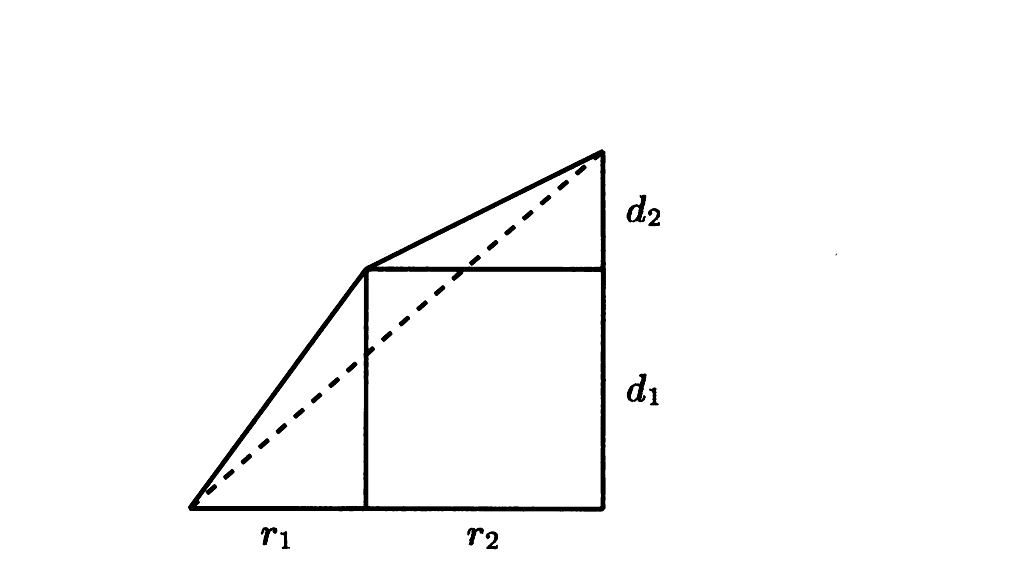
\includegraphics[width=0.45\textwidth]{figures/fig9.1.png}
    \figtitle{9.1}{跷跷板原理（原书 p.144）}
  \end{figure}

  % [Tutor Note: 背景：图 9.1 中以 $r_1,r_2$ 为宽、$d_1,d_2$ 为高作阶梯形折线与对角线，折线在直线上方当且仅当 $\mu(\cV_1)>\mu(\cV)$ 且 $\mu(\cV_2)<\mu(\cV)$。因倾斜方向如同跷跷板的两端，故称跷跷板原理。]

  \begin{align}
    \mu(\cV_1)-\mu(\cV)&=\frac{d_1}{r_1}-\frac dr \tag{9.12.13}\\
    &=\frac{d_1}{r_1}-\frac{d_1+d_2}{r_1+r_2} \tag{9.12.14}\\
    &=\frac{d_1(r_1+r_2)-r_1(d_1+d_2)}{r_1(r_1+r_2)} \tag{9.12.15}\\
    &=\frac{d_1r_2-r_1d_2}{r_1(r_1+r_2)}, \tag{9.12.16}\\
    \mu(\cV)-\mu(\cV_2)&=\frac dr-\frac{d_2}{r_2} \tag{9.12.17}\\
    &=\frac{d_1+d_2}{r_1+r_2}-\frac{d_2}{r_2} \tag{9.12.18}\\
    &=\frac{(d_1+d_2)r_2-(r_1+r_2)d_2}{(r_1+r_2)r_2} \tag{9.12.19}\\
    &=\frac{d_1r_2-r_1d_2}{(r_1+r_2)r_2}. \tag{9.12.20}
  \end{align}
\end{proof}

\begin{corollary*}{9.12.9}
  定义 9.12.5 的条件 (ii) 与下述条件等价：对任意非零的 $\cQ\subset\cE/\cE_0$，有
  \begin{equation}
    \mu(\cQ)<\mu(\cE_0).
    \tag{9.12.21}
  \end{equation}
\end{corollary*}
\begin{proof}
  选取 $\cQ\subset\cE/\cE_0$ 与选取 $\cE_0\subsetneq\cG\subsetneq\cE$，通过 $\cQ=\cG/\cE_0$ 而彼此等价。令
  \begin{equation}
    r_1:=\rank\cE_0,\quad r_2:=\rank\cQ,\quad r:=\rank\cG=r_1+r_2,
    \tag{9.12.22}
  \end{equation}
  \begin{equation}
    d_1:=\deg\cE_0,\quad d_2:=\deg\cQ,\quad d:=\deg\cG=d_1+d_2,
    \tag{9.12.23}
  \end{equation}
  则由图 9.1，

  % [原文 p.145]

  \begin{equation}
    \mu(\cG)=\frac dr<\mu(\cE_0)=\frac{d_1}{r_1}
    \tag{9.12.24}
  \end{equation}
  与
  \begin{equation}
    \mu(\cQ)=\frac{d_2}{r_2}<\mu(\cE_0)=\frac{d_1}{r_1}
    \tag{9.12.25}
  \end{equation}
  显然等价。
\end{proof}

\begin{corollary*}{9.12.10}
  对全纯向量丛的任意正合列
  \begin{equation}
    0\to\cA\to\cB\to\cC\to0
    \tag{9.12.26}
  \end{equation}
  与任意全纯向量丛 $\cD$，若 $\mu(\cD)\ge\mu(\cA)$ 且 $\mu(\cD)\ge\mu(\cC)$，则 $\mu(\cD)\ge\mu(\cB)$。
\end{corollary*}
\begin{proof}
  由跷跷板原理，
  \begin{equation}
    \mu(\cA)\le\mu(\cB)\le\mu(\cC)
    \tag{9.12.27}
  \end{equation}
  或
  \begin{equation}
    \mu(\cA)\ge\mu(\cB)\ge\mu(\cC)
    \tag{9.12.28}
  \end{equation}
  成立。主张由此立得。
\end{proof}

\begin{corollary*}{9.12.11}
  设给定全纯向量丛的序列
  \begin{equation}
    0=\cF_0\subset\cF_1\subset\cdots\subset\cF_k=\cE
    \tag{9.12.29}
  \end{equation}
  与全纯向量丛 $\cD$，且对任意 $i=1,\dots,k$ 有 $\mu(\cD)\ge\cD_i:=\cF_i/\cF_{i-1}$。此时
  \begin{equation}
    \mu(\cD)>\mu(\cE)
    \tag{9.12.30}
  \end{equation}
  成立。
\end{corollary*}
\begin{proof}
  反复应用推论 9.12.10 即可容易地得到主张。
\end{proof}

% [Tutor Note: 校勘：原书 (9.12.30) 前的不等式印作「$\mu(\cD)\ge\cD_i$」，右端脱一 $\mu$，当作 $\mu(\cD)\ge\mu(\cD_i)$；此处照原书录出。]

\begin{lemma*}{9.12.12}
  设 $\cE$ 为全纯向量丛，$\cF_1$ 与 $\cF_2$ 为 $\cE$ 的子丛。若 $\cF_1$ 半稳定、$\cF_2$ 满足条件 (9.12.21)，且 $\cF_1\subsetneq\cF_2$，则 $\mu(\cF_1)<\mu(\cF_2)$。
\end{lemma*}
\begin{proof}
  对映射 $\cF_1\to\cE/\cF_2$ 应用引理 9.12.3，得可交换图式
  \begin{equation}
    \begin{array}{ccccc}
      \cF_1&\longrightarrow&\cQ&\longrightarrow&0\\[8pt]
      \big\downarrow&&\underset{\beta}{\big\downarrow}&&\\[8pt]
      \cE/\cF_2&\longleftarrow&\cS&\longleftarrow&0
    \end{array}
    \tag{9.12.31}
  \end{equation}
% [原文 p.146]
  由 $\cF_1$ 的半稳定性有
  \begin{equation}
    \mu(\cF_1)\le\mu(\cQ),
    \tag{9.12.32}
  \end{equation}
  又由对 $\cF_2$ 的条件 (9.12.21) 得
  \begin{equation}
    \mu(\cS)<\mu(\cF_2).
    \tag{9.12.33}
  \end{equation}
  此外，由 $\det\beta\ne0$ 得 $\deg\cQ\le\deg\cS$，与 $\rank\cQ=\rank\cS$ 结合起来得
  \begin{equation}
    \mu(\cQ)\le\mu(\cS).
    \tag{9.12.34}
  \end{equation}
  因此 $\mu(\cF_1)<\mu(\cF_2)$。
\end{proof}

\begin{proof}[命题 9.12.6 的证明]
  首先证明存在性。令
  \begin{equation}
    \mu_0=\sup_{0\ne\cF\subsetneq\cE}\mu(\cF),
    \tag{9.12.35}
  \end{equation}
  则由 $\cE$ 的不稳定性得 $\mu_0>\mu(\cE)$。由于 $\mu(\cF)$ 的分母必定小于 $\rank\cE$，故 $\mu(\cF)$ 所取的值是离散的。又，对任意联络层 $\cF$ 与丰富线丛 $\cL$，$k$ 取得足够大时 $H^0(\cF\otimes\cL^{\otimes(-k)})=0$，因此子丛的次数有上界。于是 $\mu_0$ 定义中的上确界成为最大值。在满足 $\mu(\cF)=\mu_0$ 的 $\cF\subset\cE$ 中取一个 $\rank(\cF)$ 最大者，记为 $\cF$，则
  \begin{enumerate}[label=\arabic*.,leftmargin=2em,itemsep=1pt,topsep=2pt]
    \item 对任意 $\cG\subset\cF$ 有 $\mu(\cG)\le\mu(\cF)$；
    \item 对任意 $\cF\subsetneq\cG\subset\cE$ 有 $\mu(\cG)<\mu(\cF)$。
  \end{enumerate}
  前一条推出 $\cF$ 的半稳定性；后一条与系 9.12.9 一起推出定义 9.12.5 的条件 (ii)。

  其次证明唯一性。假设 $\cF_1$ 与 $\cF_2$ 都是满足定义 9.12.5 条件 (ii) 的半稳定向量丛，则只要 $\cF_1\ne\cF_2$ 就有 $\cF_1\not\subset\cF_2$ 且 $\cF_2\not\subset\cF_1$。于是由引理 9.12.12 得 $\mu(\cF_1)<\mu(\cF_2)$ 且 $\mu(\cF_2)<\mu(\cF_1)$，这不合理，因此 $\cF_1=\cF_2$。
\end{proof}

\begin{proof}[命题 9.12.7 的证明]
  对滤过长度 $k$ 作归纳来证明。$k=1$ 时主张是显然的。对一般的 $k$，由归纳假设有
  \begin{equation}
    (\cE/\cF_1)_0=\cF_2/\cF_1.
    \tag{9.12.36}
  \end{equation}
  先对 $\cE$ 的任意子丛 $\cA$ 证明
  \begin{equation}
    \mu(\cA)\le\mu(\cF_1).
    \tag{9.12.37}
  \end{equation}
  由正合列
% [原文 p.147]
  \begin{equation}
    0\to\cF_1\cap\cA\to\cA\to\cA/(\cF_1\cap\cA)\to0
    \tag{9.12.38}
  \end{equation}
  由 (9.12.36) 得
  \begin{equation}
    \mu(\cA/(\cF_1\cap\cA))\le\mu(\cF_2/\cF_1),
    \tag{9.12.39}
  \end{equation}
  再结合
  \begin{equation}
    \mu(\cF_2/\cF_1)=\mu(\cD_2)<\mu(\cD_1)=\mu(\cF_1)
    \tag{9.12.40}
  \end{equation}
  得
  \begin{equation}
    \mu(\cA/(\cF_1\cap\cA))<\mu(\cF_1).
    \tag{9.12.41}
  \end{equation}
  又由 $\cF_1$ 的半稳定性有
  \begin{equation}
    \mu(\cF_1\cap\cA)\le\mu(\cF_1).
    \tag{9.12.42}
  \end{equation}
  由 (9.12.38)、(9.12.41)、(9.12.42) 以及系 9.12.10 即得 (9.12.37)。

  其次对任意 $\cA\subset\cE$，用反证法证明：若
  \begin{equation}
    \mu(\cA)=\mu(\cF_1),
    \tag{9.12.43}
  \end{equation}
  则 $\cA\subset\cF_1$。$\cA\not\subset\cF_1$ 与 $\cA/(\cF_1\cap\cA)\ne0$ 等价。由 (9.12.42) 与 (9.12.43) 得
  \begin{equation}
    \mu(\cF_1\cap\cA)\le\mu(\cA).
    \tag{9.12.44}
  \end{equation}
  于是由正合列 (9.12.38) 与跷跷板原理得
  \begin{equation}
    \mu(\cA/(\cF_1\cap\cA))\ge\mu(\cA).
    \tag{9.12.45}
  \end{equation}
  然而
  \begin{equation}
    \mu(\cA)=\mu(\cF_1)=\mu(\cD_1)>\mu(\cD_2),
    \tag{9.12.46}
  \end{equation}
  故
  \begin{equation}
    \mu(\cA/(\cF_1\cap\cA))>\mu(\cD_2),
    \tag{9.12.47}
  \end{equation}
  这与归纳假设 (9.12.36) 矛盾。因此 $\cA\subset\cF_1$。
\end{proof}

\begin{proof}[定理 9.12.1 的证明]
  首先证明存在性。对全纯向量丛 $\cE$，若 $\cE$ 半稳定则 $k=1$，而平凡列
  \begin{equation}
    0\subset\cE
    \tag{9.12.48}
  \end{equation}
  即给出 Harder--Narasimhan 滤过。若 $\cE$ 不稳定，则
% [原文 p.148]
  记 $\cE$ 的极大不稳定化子丛为 $\cF_1$。若商丛 $\cE/\cF_1$ 半稳定，则 $k=2$，而
  \begin{equation}
    0\subset\cF_1\subset\cE
    \tag{9.12.49}
  \end{equation}
  给出 Harder--Narasimhan 滤过。若 $\cE/\cF_1$ 不稳定，则记 $\cE/\cF_1$ 的极大不稳定化子丛为 $\cD_2$，并记 $\cD_2$ 沿自然射影 $\cE\to\cE/\cF_1$ 的原像为 $\cF_2\subset\cE$。此时 $\cF_2/\cF_1\cong\cD_2$ 是半稳定的。若 $\cE/\cF_2$ 半稳定，则 $k=3$，而
  \begin{equation}
    0\subset\cF_1\subset\cF_2\subset\cE
    \tag{9.12.50}
  \end{equation}
  给出 Harder--Narasimhan 滤过。若 $\cE/\cF_2$ 不是半稳定的，则取其极大不稳定化子丛记为 $\cD_3$。反复这一操作所得的 $\cF_i$ 的秩关于 $i$ 严格单调增加，故这一操作在有限次后停止。由定义 9.12.5 的条件 (ii)，对如此得到的序列有 $\mu(\cD_1)>\mu(\cD_2)>\cdots>\mu(\cD_k)$ 成立。

  其次证明唯一性。由命题 9.12.7，滤过的首项 $\cF_1$ 是极大不稳定化子丛，故由命题 9.12.6 它唯一。滤过的次项 $\cF_2$ 是 $\cE/\cF_1$ 的极大不稳定化子丛在 $\cE$ 中的原像，故也唯一。以下同样可逐次看出：对一切 $i=1,\dots,k$，$\cF_i$ 都是唯一的。
\end{proof}

  定理 9.12.2 的证明要用到下列引理：

\begin{lemma*}{9.12.13}[Zassenhaus]
  设 $R$ 为交换环，$E$ 为 $R$ 模，$F$ 与 $G$ 为 $E$ 的子模，$F'$ 为 $F$ 的子模，$G'$ 为 $G$ 的子模，则存在自然的同构
  \begin{equation}
    (F\cap G+F')/(F\cap G'+F')\cong(F\cap G+G')/(F'\cap G+G').
    \tag{9.12.51}
  \end{equation}
\end{lemma*}
\begin{proof}
  在自然的 $R$ 模同构
  \begin{equation}
    (F\cap G+F')/F'\cong(F\cap G)/(F'\cap G)
    \tag{9.12.52}
  \end{equation}
  中，左边的子模 $F\cap G'+F'$ 对应右边的子模 $F\cap G'+F'\cap G$。因此存在 $R$ 模同构
  \begin{equation}
    (F\cap G+F')/(F\cap G'+F')\cong(F\cap G)/(F\cap G'+F'\cap G).
    \tag{9.12.53}
  \end{equation}
  同样地，
% [原文 p.149]
  \begin{equation}
    (F\cap G+G')/(F'\cap G+G')\cong(F\cap G)/(F\cap G'+F'\cap G),
    \tag{9.12.54}
  \end{equation}
  由 (9.12.53) 与 (9.12.54) 立即得到 (9.12.51)。
\end{proof}

\begin{corollary}{9.12.14}
  设 $X$ 为 Riemann 面，$\cE$ 为 $X$ 上的全纯向量丛，$\cF$ 与 $\cG$ 为 $\cE$ 的全纯子丛，$\cF'$ 为 $\cF$ 的全纯子丛，$\cG'$ 为 $\cG$ 的全纯子丛，则存在自然的同构
  \begin{equation}
    (\cF\cap\cG+\cF')/(\cF\cap\cG'+\cF')\cong(\cF\cap\cG+\cG')/(\cF'\cap\cG+\cG').
    \tag{9.12.55}
  \end{equation}
\end{corollary}

\begin{lemma*}{9.12.15}
  设 $\cE$ 为 Riemann 面上的全纯向量丛，$\cF$ 为 $\cE$ 的全纯子丛。若 $\cE$ 半稳定，且 $\cE$ 与 $\cF$ 的梯度相等，则 $\cF$ 也半稳定。
\end{lemma*}
\begin{proof}
  由 $\cF$ 的全纯子丛也是 $\cE$ 的全纯子丛以及半稳定性的定义，主张立即得到。
\end{proof}

\begin{lemma*}{9.12.16}
  设 $X$ 为 Riemann 面，$\cE$ 为 $X$ 上的全纯向量丛，$\cF$ 与 $\cG$ 为 $\cE$ 的全纯子丛。若 $\cE$、$\cF$ 以及 $\cG$ 都是梯度为 $\mu$ 的半稳定向量丛，则 $\cF+\cG$ 与 $\cF\cap\cG$ 也都是梯度为 $\mu$ 的半稳定向量丛。
\end{lemma*}
\begin{proof}
  由于 $\cF+\cG$ 是 $\cE$ 的全纯子丛，
  \begin{equation}
    \mu(\cF+\cG)\le\mu(\cE)=\mu.
    \tag{9.12.56}
  \end{equation}
  另一方面，$\cF$ 与 $\cG$ 是梯度相等的半稳定丛，故 $\cF\oplus\cG$ 也半稳定。由正合列
  \begin{equation}
    0\to\cF\cap\cG\to\cF\oplus\cG\to\cF+\cG\to0
    \tag{9.12.57}
  \end{equation}
  得
  \begin{equation}
    \mu(\cF+\cG)\ge\mu(\cF\oplus\cG)=\mu,
    \tag{9.12.58}
  \end{equation}
  于是归结为
  \begin{equation}
    \mu(\cF\cap\cG)=\mu(\cF+\cG)=\mu.
    \tag{9.12.59}
  \end{equation}
  因此，由引理 9.12.15，$\cF\cap\cG$ 与 $\cF+\cG$ 也都半稳定。
\end{proof}

% [原文 p.150]
\begin{proof}[定理 9.12.2 的证明]
  设给定半稳定向量丛 $\cE$ 的两个 Jordan--Hölder 滤过
  \begin{equation}
    0\subset\cF_1\subset\cF_2\subset\cdots\subset\cF_k=\cE
    \tag{9.12.60}
  \end{equation}
  与
  \begin{equation}
    0\subset\cG_1\subset\cG_2\subset\cdots\subset\cG_l=\cE,
    \tag{9.12.61}
  \end{equation}
  并令
  \begin{align}
    \cF_{i,j}&:=\cF_{i+1}\cap\cG_j+\cF_i, \tag{9.12.62}\\
    \cG_{i,j}&:=\cF_i\cap\cG_{j+1}+\cG_j. \tag{9.12.63}
  \end{align}
  此时
  \begin{align}
    \cF_i=\cF_{i,0}\subset\cF_{i,1}\subset\cdots\subset\cF_{i,l}=\cF_{i+1}, \tag{9.12.64}\\
    \cG_j=\cG_{0,j}\subset\cG_{1,j}\subset\cdots\subset\cG_{k,j}=\cG_{j+1} \tag{9.12.65}
  \end{align}
  成立；而由 $\cF_{i,j}$ 与 $\cG_{i,j}$ 的半稳定性以及 $\cF_i/\cF_{i+1}$ 与 $\cG_j/\cG_{j+1}$ 的稳定性，这些滤过的包含映射除一处之外都是同构。由系 9.12.14 得
  \begin{align}
    \cF_{i,j}/\cF_{i,j-1}
    &=\bigl(\cF_{i+1}\cap\cG_j+\cF_i\bigr)\big/\bigl(\cF_{i+1}\cap\cG_{j-1}+\cF_i\bigr) \tag{9.12.66}\\
    &\cong\bigl(\cF_{i+1}\cap\cF_j+\cG_{j-1}\bigr)\big/\bigl(\cF_i\cap\cG_j+\cG_{j-1}\bigr) \tag{9.12.67}\\
    &=\cG_{i+1,j-1}/\cG_{i,j-1}, \tag{9.12.68}
  \end{align}
  这意味着逐次商的列在调换顺序后一致。
\end{proof}

% [Tutor Note: 校勘：原书 p.150 行内两处下标疑倒置。其一印作「$\cF_i/\cF_{i+1}$ 与 $\cG_j/\cG_{j+1}$ 的稳定性」，因 $\cF_i\subset\cF_{i+1}$ 而应为 $\cF_{i+1}/\cF_i$、$\cG_{j+1}/\cG_j$；其二 (9.12.67) 分子第二项印作 $\cF_j$，按 Zassenhaus 引理 (9.12.55) 应为 $\cG_j$。此处照原书录出。]

\section{常中心曲率 Hermite 度量的唯一性}

任意复化规范变换 $\tilde g\in\cG_{\C}$，按各点处的 Cartan 分解，都可写成正定 Hermite 矩阵值的复规范变换 $g$ 与酉规范变换 $u$ 之积：
\begin{equation}
  \tilde g=g\cdot u,\qquad g=g^*,\qquad u\in\cG.
  \tag{9.13.1}
\end{equation}
酉规范变换 $u$ 不改变联络的同型类，故可设 $\tilde g=g$。由 (9.7.7)，由这样的 $g$ 给出的规范变换，在令
\begin{equation}
  \alpha=\bigl(\overline{\partial}_Ag\bigr)g^{-1}
  \tag{9.13.2}
\end{equation}
时，由下式给出：
% [原文 p.151]
\begin{equation}
  g(A)=A+\alpha^*-\alpha.
  \tag{9.13.3}
\end{equation}
此时由 (9.2.21) 得
\begin{equation}
  F_{g(A)}=F_A+d_A(\alpha^*-\alpha)+(\alpha^*-\alpha)\wedge(\alpha^*-\alpha).
  \tag{9.13.4}
\end{equation}
复规范群的作用把 $\cA^{1,1}\subset\cA$ 的元素仍映到 $\cA^{1,1}$，故 $F_{g(A)}$ 是 $(1,1)$ 形式。由于 $\alpha$ 与 $\alpha^*$ 分别是 $(0,1)$ 形式与 $(1,0)$ 形式，给出 $F_{g(A)}$ 的 $(2,0)$ 分量与 $(0,2)$ 分量的 $\partial_A\alpha^*$、$\alpha\wedge\alpha$ 等项不必计算也会相消，因此
\begin{equation}
  F_{g(A)}=F_A+\overline{\partial}_A\alpha^*-\partial_A\alpha-\alpha^*\wedge\alpha-\alpha\wedge\alpha^*.
  \tag{9.13.5}
\end{equation}
成立。又

\begin{align}
  \alpha^*&=\bigl((\overline{\partial}_Ag)g^{-1}\bigr)^* \tag{9.13.6}\\
  &=(g^{-1})^*\partial_Ag^* \tag{9.13.7}\\
  &=g^{-1}\partial_Ag, \tag{9.13.8}
\end{align}
故
\begin{align}
  F_{g(A)}-F_A
  &=\overline{\partial}_A\bigl(g^{-1}\partial_Ag\bigr)-\partial_A\bigl((\overline{\partial}_Ag)g^{-1}\bigr) \notag\\
  &\quad-g^{-1}\partial_Ag\wedge(\overline{\partial}_Ag)g^{-1}-(\overline{\partial}_Ag)g^{-1}\wedge g^{-1}\partial_Ag \notag\\
  &=-g^{-1}(\overline{\partial}_Ag)g^{-1}(\partial_Ag)+g^{-1}(\overline{\partial}_A\partial_Ag) \notag\\
  &\quad-(\partial_A\overline{\partial}_Ag)g^{-1}-(\overline{\partial}_Ag)g^{-1}(\partial_Ag)g^{-1} \notag\\
  &\quad-g^{-1}\partial_Ag\wedge(\overline{\partial}_Ag)g^{-1}-(\overline{\partial}_Ag)g^{-1}\wedge g^{-1}\partial_Ag. \tag{9.13.9}
\end{align}

\begin{lemma*}{9.13.1}
  $F_{g(A)}=F_A$ 的充要条件是
  \begin{equation}
    \partial_A\overline{\partial}_A(g^2)
    =-\bigl\{(\overline{\partial}_A(g^2))g^{-1}\bigr\}\bigl\{(\overline{\partial}_A(g^2))g^{-1}\bigr\}^*
    +[F_A,g]g.
    \tag{9.13.10}
  \end{equation}
\end{lemma*}
\begin{proof}
  反复使用 Leibniz 法则，(9.13.10) 的左端可表为
  \begin{align*}
    &\partial_A\bigl((\overline{\partial}_Ag)g+g(\overline{\partial}_Ag)\bigr)\\
    &\quad=(\partial_A\overline{\partial}_Ag)g-(\overline{\partial}_Ag)(\partial_Ag)+(\partial_Ag)(\overline{\partial}_Ag)+g(\partial_A\overline{\partial}_Ag).
  \end{align*}
  另一方面，(9.13.10) 右端第 1 项变号后为
% [原文 p.152]
  \begin{align*}
    &\bigl(\{(\overline{\partial}_Ag)g+g(\overline{\partial}_Ag)\}g^{-1}\bigr)
     \bigl(\{(\overline{\partial}_Ag)g+g(\overline{\partial}_Ag)\}g^{-1}\bigr)^*\\
    &\quad=\bigl\{\overline{\partial}_Ag+g(\overline{\partial}_Ag)g^{-1}\bigr\}
      \bigl\{\overline{\partial}_Ag+g(\overline{\partial}_Ag)g^{-1}\bigr\}^*\\
    &\quad=\bigl\{\overline{\partial}_Ag+g(\overline{\partial}_Ag)g^{-1}\bigr\}
      \bigl\{\partial_Ag+g^{-1}(\partial_Ag)g\bigr\}\\
    &\quad=(\overline{\partial}_Ag)(\partial_Ag)+(\overline{\partial}_Ag)g^{-1}(\partial_Ag)g\\
    &\qquad+g(\overline{\partial}_Ag)g^{-1}(\partial_Ag)+g(\overline{\partial}_Ag)g^{-2}(\partial_Ag)g.
  \end{align*}
  成立。因此从 (9.13.10) 的左端减去右端第 1 项得
  \begin{align*}
    &(\partial_A\overline{\partial}_Ag)g+(\overline{\partial}_Ag)(\overline{\partial}_Ag)+g(\partial_A\overline{\partial}_Ag)+(\overline{\partial}_Ag)g^{-1}(\overline{\partial}_Ag)g\\
    &\qquad+g(\overline{\partial}_Ag)g^{-1}(\overline{\partial}_Ag)+g(\overline{\partial}_Ag)g^{-2}(\overline{\partial}_Ag)g.
  \end{align*}
  在此式上再加上把 (9.13.9) 的右端左右两侧乘以 $g$ 所得的式子，即得
  \begin{equation}
    \bigl((\partial_A\overline{\partial}_A+\overline{\partial}_A\partial_A)g\bigr)g=[F_A,g]g.
    \tag{9.13.11}
  \end{equation}
\end{proof}

  这里，注意到对任意复矩阵 $A=(A_{ij})_{i,j=1}^n$ 有
  \begin{equation}
    \tr(A\,d\bar z\wedge A^*dz)=-\tr(AA^*)\,dz\wedge d\bar z,
    \tag{9.13.12}
  \end{equation}
  \begin{equation}
    \tr(AA^*)=\sum_{i,j=1}^n|A_{ij}|^2\ge0
    \tag{9.13.13}
  \end{equation}
  以及
  \begin{equation}
    \partial\overline{\partial}\colon\Omega^0(X)\to\Omega^{1,1}(X)
    \tag{9.13.14}
  \end{equation}
  用 $X$ 上的局部坐标 $z=x+\sqrt{-1}\,y$ 给出为
  \begin{align}
    \partial\overline{\partial}f&=(\partial_z\overline{\partial}_zf)\,dz\wedge d\bar z \tag{9.13.15}\\
    &=\frac14\biggl(\frac{\partial^2}{\partial x^2}+\frac{\partial^2}{\partial y^2}\biggr)f\,dz\wedge d\bar z, \tag{9.13.16}
  \end{align}
  对 (9.13.10) 的两端取迹，利用迹的循环不变性带来的
  \begin{equation}
    \tr([F_A,g]g)=0
    \tag{9.13.17}
  \end{equation}
  以及对任意 $\varphi\in\Gamma(P\times_G\mathfrak{g})$ 成立的
  \begin{equation}
    \partial\overline{\partial}\tr(\varphi)=\tr(\partial_A\overline{\partial}_A\varphi),
    \tag{9.13.18}
  \end{equation}
  则由下面的最大值原理（maximum principle）可知 $\tau:=\tr g^2$ 为常数。
% [原文 p.153]
\takeaway{复规范变换后曲率不变的充要条件是 (9.13.10)；其迹给出 $\tau=\tr g^2$ 满足最大值原理，故 $\tau$ 为常数，再由稳定性得 $g$ 为常数标量，唯一性随之成立。}

\begin{theorem}{9.13.2（最大值原理）}
  设 $U$ 为 $\R^m$ 中的区域，$(g_{ij})_{i,j=1}^m$ 为取 $m$ 次正定对称矩阵值的 $U$ 上的 $C^\infty$ 函数，$(h_i)_{i=1}^m$ 为 $U$ 上的 $C^\infty$ 函数。此时，若 $U$ 上的 $C^\infty$ 函数 $f$ 满足不等式
  \begin{equation}
    \sum_{i,j=1}^n g_{ij}\frac{\partial^2f}{\partial x_i\partial x_j}
    +\sum_{i=1}^m h_i\frac{\partial f}{\partial x_i}\ge0
    \tag{9.13.19}
  \end{equation}
  且 $f$ 在 $U$ 的内点取得最大值，则 $f$ 是常数。
\end{theorem}

% [Tutor Note: 校勘：原书 (9.13.19) 第一项求和下标印作 $i,j=1,\dots,n$，而 $g_{ij}$ 为 $m$ 次矩阵、区域在 $\R^m$ 中，当为 $i,j=1,\dots,m$；此处照原书录出。]

最大值原理的详细论述例如可参见 [44, 6.4 节]。对任意复矩阵 $A=(\overline{\partial}_Ag^2)g^{-1}$，$\tr(AA^*)=0$ 与 $A=0$ 等价，故由 $\partial\overline{\partial}\tau=0$ 得
\begin{equation}
  (\overline{\partial}_Ag^2)g^{-1}=0,
  \tag{9.13.20}
\end{equation}
即
\begin{equation}
  \overline{\partial}_Ag^2=0.
  \tag{9.13.21}
\end{equation}
因此 $g^2$ 给出 $\cE$ 的全纯自同构，而 $\cE$ 稳定，从而特别地单纯，故 $g^2$ 必须是常数标量。于是 $A=g(A)$，唯一性得证。

\section{Hermite 矩阵的范数}

记 $r$ 次 Hermite 矩阵构成的实线性空间为 $H=H_r$。$H$ 上的范数
\begin{equation}
  \nu\colon H\to\R^{\ge0}
  \tag{9.14.1}
\end{equation}
定义为
\begin{equation}
  \nu(M)=\tr\bigl((M^*M)^{\frac12}\bigr).
  \tag{9.14.2}
\end{equation}

\begin{lemma*}{9.14.1}
  $\nu$ 与 $H$ 的通常范数
  \begin{equation}
    \|M\|_H=\bigl(\tr(M^*M)\bigr)^{\frac12}
    \tag{9.14.3}
  \end{equation}
  等价。
\end{lemma*}
\begin{proof}
  用酉矩阵 $U\in U(r)$ 把 $M\in H$ 对角化为
  \begin{equation}
    M=U^*\operatorname{diag}(\lambda_1,\dots,\lambda_r)U,
    \tag{9.14.4}
  \end{equation}
  则
% [原文 p.154]
  \begin{align*}
    M^*M&=(U^*\operatorname{diag}(\lambda_1,\dots,\lambda_r)U)^*(U^*\operatorname{diag}(\lambda_1,\dots,\lambda_r)U)\\
    &=U^*\operatorname{diag}(\lambda_1,\dots,\lambda_r)UU^*\operatorname{diag}(\lambda_1,\dots,\lambda_r)U\\
    &=U^*\operatorname{diag}(\lambda_1^2,\dots,\lambda_r^2)U,\\
    (M^*M)^{\frac12}&=U^*\operatorname{diag}(|\lambda_1|,\dots,|\lambda_r|)U.
  \end{align*}
  故
  \begin{equation}
    \nu(M)=\sum_{i=1}^r|\lambda_i|,
    \tag{9.14.5}
  \end{equation}
  \begin{equation}
    \|M\|_H=\biggl(\sum_{i=1}^r\lambda_i^2\biggr)^{\frac12}
    \tag{9.14.6}
  \end{equation}
  成立。关于范数 $\nu$ 的单位球面由
  \begin{equation}
    |\lambda_1|+|\lambda_2|+\cdots+|\lambda_r|=1
    \tag{9.14.7}
  \end{equation}
  定义。在 $\lambda$ 空间的第 1 象限内，它是 $r-1$ 维的标准单形；整体上则是把它关于各坐标超平面折返所得的 $2^r$ 个图形的并集。由于关于范数 $\nu$ 的单位球面完全含于关于范数 $\|\cdot\|_H$ 的单位球体内，故对任意 $M\in H$ 有
  \begin{equation}
    \|M\|_H\le\nu(M).
    \tag{9.14.8}
  \end{equation}
  另一方面，范数 $\nu$ 与范数 $\|\cdot\|_H$ 之差最大是在 $\lambda_1=\cdots=\lambda_r=\lambda$ 时，此时
  \begin{equation}
    \|\operatorname{diag}(\lambda,\dots,\lambda)\|_H=\sqrt r\,|\lambda|,
    \tag{9.14.9}
  \end{equation}
  \begin{equation}
    \nu(\operatorname{diag}(\lambda,\dots,\lambda))=r|\lambda|
    \tag{9.14.10}
  \end{equation}
  成立。因此
  \begin{equation}
    \nu(M)\le\sqrt r\,\|M\|_H.
    \tag{9.14.11}
  \end{equation}
\end{proof}

\takeaway{$\nu$ 与 Hilbert--Schmidt 范数 $\|\cdot\|_H$ 等价，且 $\|M\|_H\le\nu(M)\le\sqrt r\|M\|_H$。}

记 $\C^r$ 的标准正交基全体构成的集合为
\begin{equation}
  O=\bigl\{(e_i)_{i=1}^r\bigm|(e_i)_{i=1}^r \text{ 是 } \C^r \text{ 的标准正交基}\bigr\},
  \tag{9.14.12}
\end{equation}
则 $O$ 自然地与酉群 $U(r)$ 等同。

\begin{lemma*}{9.14.2}
  对任意 $M\in H$ 有
  \begin{equation}
    \nu(M)=\max_{(e_i)_{i=1}^r\in O}\sum_{i=1}^r\bigl|(Me_i,e_i)\bigr|.
    \tag{9.14.13}
  \end{equation}
\end{lemma*}

% [原文 p.155]
\begin{proof}
  适当选取 $\C^r$ 的坐标，可设 $M$ 为对角矩阵：
  \begin{equation}
    M=\operatorname{diag}(\lambda_1,\dots,\lambda_r).
    \tag{9.14.14}
  \end{equation}
  用坐标把 $O$ 的元素 $(e_i)_{i=1}^r$ 写成
  \begin{equation}
    e_i=(e_{i1},\dots,e_{ir}),\qquad i=1,\dots,r,
    \tag{9.14.15}
  \end{equation}
  则
  \begin{align}
    \bigl|(Me_i,e_i)\bigr|
    &=\bigl|\bigl((\lambda_1e_{i1},\dots,\lambda_re_{ir}),(e_{i1},\dots,e_{ir})\bigr)\bigr| \tag{9.14.16}\\
    &=\bigl\lvert\lambda_1\lvert e_{i1}\rvert^2+\cdots+\lambda_r\lvert e_{ir}\rvert^2\bigr\rvert \tag{9.14.17}\\
    &\le|\lambda_1||e_{i1}|^2+\cdots+|\lambda_r||e_{ir}|^2 \tag{9.14.18}\\
    &=\sum_{j=1}^r|\lambda_j||e_{ij}|^2. \tag{9.14.19}
  \end{align}
  故
  \begin{align}
    \sum_{i=1}^r\bigl|(Me_i,e_i)\bigr|
    &\le\sum_{i=1}^r\sum_{j=1}^r|\lambda_j||e_{ij}|^2 \tag{9.14.20}\\
    &=\sum_{j=1}^r|\lambda_j|\sum_{i=1}^r|e_{ij}|^2 \tag{9.14.21}\\
    &=\sum_{j=1}^r|\lambda_j|, \tag{9.14.22}
  \end{align}
  从而
  \begin{equation}
    \nu(M)\ge\max_{(e_i)_{i=1}^r\in O}\sum_{i=1}^r\bigl|(Me_i,e_i)\bigr|.
    \tag{9.14.23}
  \end{equation}
  另一方面，取 $(e_i)_{i=1}^r$ 为坐标基，则
  \begin{equation}
    \nu(M)=\sum_{i=1}^r\bigl|(Me_i,e_i)\bigr|
    \tag{9.14.24}
  \end{equation}
  成立，故
  \begin{equation}
    \nu(M)\le\max_{(e_i)_{i=1}^r\in O}\sum_{i=1}^r\bigl|(Me_i,e_i)\bigr|.
    \tag{9.14.25}
  \end{equation}
\end{proof}

% [Tutor Note: 校勘：原书 (9.14.17) 内层印作「$|\lambda_1|e_{i1}|^2+\cdots+\lambda_r|e_{ir}|^2|$」，其中 $\lambda_r$ 外脱绝对值符号；因 $\lambda_j$ 为实特征值且外层取绝对值，结果不受影响，此处照原书录出。]

由引理 9.14.2 得下列系：

% [原文 p.156]
\begin{corollary*}{9.14.3}
  当矩阵 $M$ 为形如
  \begin{equation}
    M=\begin{pmatrix}A&B\\C&D\end{pmatrix}
    \tag{9.14.26}
  \end{equation}
  的分块矩阵时，
  \begin{equation}
    \nu(M)\ge|\tr A|+|\tr D|
    \tag{9.14.27}
  \end{equation}
  成立。
\end{corollary*}
\begin{proof}
  取 $(e_i)_{i=1}^r$ 为 $\C^r$ 的标准基，得
  \begin{equation}
    \nu(M)\ge\sum_{i=1}^r|M_{ii}|
    =\sum_{i=1}^{r_1}|M_{ii}|+\sum_{i=r_1+1}^r|M_{ii}|
    =|\tr A|+|\tr D|.
    \tag{9.14.28}
  \end{equation}
\end{proof}

下列系由 (9.14.5) 立即得到：

\begin{lemma}{9.14.4}
  当矩阵 $M$ 的特征值全为正时
  \begin{equation}
    \nu(M)=\tr M,
    \tag{9.14.29}
  \end{equation}
  全为负时
  \begin{equation}
    \nu(M)=-\tr M.
    \tag{9.14.30}
  \end{equation}
\end{lemma}

\section{从稳定性到常中心曲率联络}

本节的目标是证明下述定理：

\begin{theorem}{9.15.1}
  若 Riemann 面 $X$ 上的全纯向量丛 $\cE$ 稳定，则 $\cE$ 具有常中心曲率联络。
\end{theorem}

对 $\Gamma(P\times_G\mathfrak{g})$ 的元素 $s$，令
\begin{equation}
  N(s)=\biggl(\int_X\nu(s)^2\,d\mathrm{vol}_X\biggr)^{\frac12},
  \tag{9.15.1}
\end{equation}
则由引理 9.14.1，$N$ 可延拓为 $L^2(P\times_G\mathfrak{g})$ 上与 $L^2$ 范数 $\|\cdot\|_{L^2}$ 等价的范数。定义泛函 $J\colon\cA^2_1\to\R$ 为
\begin{equation}
  J(A)=N\Bigl(\frac1{2\pi\sqrt{-1}}\ast F_A+\mu\Bigr).
  \tag{9.15.2}
\end{equation}
该泛函显然有下界，故有下确界。取使下确界达到的联络列 $\{A_i\}_{i=1}^\infty$，则

% [原文 p.157]
\begin{align}
  \|F\|_{L^2}&=\|\ast F\|_{L^2} \tag{9.15.3}\\
  &=2\pi\biggl\|\frac{\ast F}{2\pi\sqrt{-1}}\biggr\|_{L^2} \tag{9.15.4}\\
  &=2\pi\biggl\|\Bigl(\frac{\ast F}{2\pi\sqrt{-1}}+\mu\Bigr)-\mu\biggr\|_{L^2} \tag{9.15.5}\\
  &\le2\pi\biggl\|\frac{\ast F}{2\pi\sqrt{-1}}+\mu\biggr\|_{L^2}+2\pi\mu \tag{9.15.6}\\
  &\le2\pi N\Bigl(\frac{\ast F}{2\pi\sqrt{-1}}+\mu\Bigr)+2\pi\mu, \tag{9.15.7}
\end{align}
因此其曲率的 $L^2$ 范数有上界。

\takeaway{用泛函 $J(A)=N\bigl(\frac{\ast F_A}{2\pi\sqrt{-1}}+\mu\bigr)$ 的极小化列、Uhlenbeck 紧性以及弱解的正则性，可由 $\cE$ 的稳定性得出常中心曲率联络的存在性。}

下述定理称为 \textbf{Uhlenbeck 紧性}（Uhlenbeck compactness），是规范理论研究中必定用到的基本定理：

\begin{theorem}{9.15.2（Uhlenbeck [132, Theorem 1.5]）}
  对 $L^2_1$ 联络的列 $\{A_i\}_{i=1}^\infty$，若其曲率的 $L^2$ 范数有上界，则存在适当的部分列 $\{A_{i_k}\}_{k=1}^\infty$ 与 $L^2_2$ 规范变换的列 $\{g_k\}_{k=1}^\infty$，使得 $\{g_k(A_{i_k})\}_{k=1}^\infty$ 在 $\cA^2_1$ 中弱收敛。
\end{theorem}

由定理 9.15.2，适当取部分列并作规范变换后，可设给出下确界的列在 $L^2_1$ 中弱收敛。于是只需证明：

\begin{enumerate}[label=\arabic*.,leftmargin=2em,itemsep=1pt,topsep=2pt]
  \item 若弱收敛极限不在 $\cG_{\C}$ 轨道中，则 $\cE$ 不稳定。
  \item 若弱收敛极限在 $\cG_{\C}$ 轨道中，则该联络具有常中心曲率。
  \item 具有常中心曲率的 $L^2_1$ 联络，经适当的 $L^2_2$ 规范变换后可变为光滑的。
\end{enumerate}

3 是椭圆型偏微分方程论中著名的椭圆正则性（elliptic regularity）在规范理论中的类似物，它也由 Uhlenbeck 给出：

\begin{theorem}{9.15.3（Uhlenbeck [Corollary 1.4]）}
  若 $L^2_1$ 联络 $A$ 满足 Yang--Mills 方程 $D\ast F=0$，则经适当的 $L^2_2$ 规范变换可成为 $C^\infty$ 级联络。
\end{theorem}

为证明 2，回忆下述定理：

\begin{theorem}{9.15.4（Hodge--de Rham--小平）}
  设给定紧流形 $X$ 上的带度量向量丛 $E_1$ 与 $E_2$，以及其截面空间之间的椭圆型线性微分算子 $P\colon\Gamma(E_1)\to\Gamma(E_2)$。此时 $\Ker P$ 与 $\Ker P^*$ 都是有限维的，且对任意 $\beta\in(\Ker P^*)^\perp\subset\Gamma(E_2)$，存在唯一的 $\varphi\in(\Ker P)^\perp\subset\Gamma(E_1)$ 使 $P\varphi=\beta$。
\end{theorem}

% [Tutor Note: 背景：原文以 $\mathcal{O}(\cE)$ 记 $\cE$ 上联络在复规范群 $\cG_{\C}$ 下的轨道（orbit），$J|_{\mathcal{O}(\cE)}$ 表示 $J$ 在该轨道上的限制；下文 9.15、9.16 各处的 $\mathcal{O}(\cE)$ 同此。]

其证明例如可参见 [135, 6 章]。用它可证明 2：

\begin{proposition*}{9.15.5}
  若存在 $A\in\mathcal{O}(\cE)$ 使
  \begin{equation}
    J(A)=\inf J|_{\mathcal{O}(\cE)}
    \tag{9.15.8}
  \end{equation}
  成立，则 $A$ 是常中心曲率联络。
\end{proposition*}
% [原文 p.158]
\begin{proof}
  把定理 9.15.4 用于 $E_1=E_2=\End E$ 以及 $P=d_A^*d_A=P^*$。$P$ 的核是 $\cE$ 的全纯自同构构成的空间，而 $\cE$ 稳定，从而特别地单纯，故全纯自同构只能是常数标量。因此 $\Ker P=\C\cdot\id_E$，而由
  \begin{align}
    \int_X\tr\bigl(2\pi\mu-\sqrt{-1}\ast F_A\bigr)
    &=2\pi\deg(\cE)-\sqrt{-1}\int\tr F_A \notag\\
    &=0
    \tag{9.15.9}
  \end{align}
  可知 $2\pi\mu-\sqrt{-1}\ast F_A$ 与 $\id_E$ 正交。于是存在 $h\in\Gamma(\End E)$ 使
  \begin{equation}
    d_A^*d_Ah=2\pi\mu-\sqrt{-1}\ast F_A.
    \tag{9.15.10}
  \end{equation}
  这里，对 $t\in\C$ 令 $g=1+th$，只要 $|t|$ 足够小，它就给出 $\cG_{\C}$ 的元素。此时，注意到
  \begin{equation}
    \partial_Ag=t\partial_Ah,\qquad \overline{\partial}_Ag=t\overline{\partial}_Ah
    \tag{9.15.11}
  \end{equation}
  关于 $t$ 是一次式，以及
  \begin{equation}
    g^{-1}=1-th+O(t^2),
    \tag{9.15.12}
  \end{equation}
  由 (9.13.9) 得
  \begin{align}
    F_{g(A)}-F_A
    &=\overline{\partial}_A\bigl(g^{-1}\partial_Ag\bigr)-\partial_A\bigl((\overline{\partial}_Ag)g^{-1}\bigr) \notag\\
    &\quad-g^{-1}\partial_Ag\wedge(\overline{\partial}_Ag)g^{-1}-(\overline{\partial}_Ag)g^{-1}\wedge g^{-1}\partial_Ag \notag\\
    &=t\bigl(\overline{\partial}_A\partial_A-\partial_A\overline{\partial}_A\bigr)h+O(t^2).
    \tag{9.15.13}
  \end{align}
  这里用到恒等式
  \begin{align*}
    d_A^*d_A&=\bigl(\partial_A^*+\overline{\partial}_A^*\bigr)\bigl(\partial_A+\overline{\partial}_A\bigr)\\
    &=\partial_A^*\partial_A+\overline{\partial}_A^*\overline{\partial}_A\\
    &=\sqrt{-1}[\Lambda,\overline{\partial}_A]\partial_A-\sqrt{-1}[\Lambda,\partial_A]\overline{\partial}_A\\
    &=\sqrt{-1}\Lambda\overline{\partial}_A\partial_A-\sqrt{-1}\Lambda\partial_A\overline{\partial}_A\\
    &=\sqrt{-1}\Lambda\bigl(\overline{\partial}_A\partial_A-\partial_A\overline{\partial}_A\bigr)\\
    &=\sqrt{-1}\ast\bigl(\overline{\partial}_A\partial_A-\partial_A\overline{\partial}_A\bigr),
  \end{align*}
% [原文 p.159]
  则
  \begin{align*}
    &N\Bigl(\frac{\ast F_{g(A)}}{2\pi\sqrt{-1}}+\mu\Bigr)\\
    &\quad=N\biggl(\frac{\ast\bigl(F_A+t(\overline{\partial}_A\partial_A-\partial_A\overline{\partial}_A)h\bigr)}{2\pi\sqrt{-1}}+\mu\biggr)+O(t^2)\\
    &\quad=N\Bigl(\frac{\ast F_A}{2\pi\sqrt{-1}}-\frac t{2\pi}d_A^*d_Ah+\mu\Bigr)+O(t^2)\\
    &\quad=N\Bigl(\frac{\ast F_A}{2\pi\sqrt{-1}}-\frac t{2\pi}\bigl(2\pi\mu-\sqrt{-1}\ast F_A\bigr)+\mu\Bigr)+O(t^2)\\
    &\quad=N\Bigl(\frac{\ast F_A}{2\pi\sqrt{-1}}+\mu\Bigr)(1-t)+O(t^2).
  \end{align*}
  因此，为使 $J_{g(A)}$ 在 $t=0$ 处取最小值，
  \begin{equation}
    \frac{\ast F_A}{2\pi\sqrt{-1}}+\mu=0
    \tag{9.15.14}
  \end{equation}
  是必要的。
\end{proof}

为证明 1，先作些准备。设给定全纯向量丛的正合列
\begin{equation}
  0\to\cS\to\cE\to\cQ\to0.
  \tag{9.15.15}
\end{equation}
$C^\infty$ 级向量丛的正合列必定分裂，故把 $\cE$ 作为 $C^\infty$ 级向量丛分解为 $\cS$ 与 $\cQ$ 的直和时，关于这一分解，$\cE$ 的酉联络可表为
\begin{equation}
  A_{\cE}=A(\cS,\cQ,\beta)
  =\begin{pmatrix}A_{\cS}&\beta<本地路径>*&A_{\cQ}\end{pmatrix},
  \tag{9.15.16}
\end{equation}
其中 $A_{\cS}$ 与 $A_{\cQ}$ 分别是 $\cS$ 与 $\cQ$ 的联络，而 $\beta\in\Omega^{0,1}(\cQ^*\otimes\cS)$ 是全纯列 (9.15.15) 的扩张类
\begin{equation}
  [\beta]\in H^1(\cQ^*\otimes\cS)\cong\Ext^1(\cQ,\cS)
  \tag{9.15.17}
\end{equation}
的代表元。此时，$A$ 的曲率为
\begin{equation}
  \begin{aligned}
    F(A_{\cE})&=dA_{\cE}+A_{\cE}\wedge A_{\cE}\\
    &=\begin{pmatrix}
      F(A_{\cS})-\beta\wedge\beta^* & d\beta+A_{\cS}\wedge\beta+\beta\wedge A_{\cQ}\\
      -d\beta^*-\beta^*\wedge A_{\cS}^*-A_{\cQ}^*\wedge\beta^* & F(A_{\cQ})-\beta^*\wedge\beta
    \end{pmatrix}.
  \end{aligned}
  \tag{9.15.18}
\end{equation}
这里 $d\beta+A_{\cS}\wedge\beta+\beta\wedge A_{\cQ}=d_{\cQ^*\otimes\cS}\beta$，是把 $\cS$ 的联络 $A_{\cS}$ 与 $\cQ$ 的联络 $A_{\cQ}$ 在 $\cQ^*\otimes\cS$ 上诱导的联络用于对 $\beta$ 微分所得。用局部坐标把 $\beta$ 表为 $\beta=B\,d\bar z$，则
\begin{equation}
  \beta^*\wedge\beta=B^*B\,dz\wedge d\bar z,
  \tag{9.15.19}
\end{equation}
而 $B^*B$ 是正定的，故可把 $\cQ^*\otimes\cS$ 的 Hermite 度量 $|\cdot|$ 取为
\begin{equation}
  \ast\tr(\beta^*\wedge\beta)=-2\pi\sqrt{-1}|\beta|^2,
  \tag{9.15.20}
\end{equation}
% [原文 p.160]
由此可以定义。此时由
\begin{equation}
  \beta\wedge\beta^*=BB^*\,d\bar z\wedge dz=-BB^*\,dz\wedge d\bar z
  \tag{9.15.21}
\end{equation}
得
\begin{equation}
  \tr(\beta\wedge\beta^*)=2\pi\sqrt{-1}|\beta|^2.
  \tag{9.15.22}
\end{equation}
对全纯向量丛的正合列 (9.15.15)，令
\begin{align*}
  J_0(\cS,\cE,\cQ)&:=\rank\cS\bigl(\mu(\cS)-\mu(\cE)\bigr)+\rank\cQ\bigl(\mu(\cE)-\mu(\cQ)\bigr),\\
  J_1(\cS,\cE,\cQ)&:=\rank\cS\bigl(\mu(\cE)-\mu(\cS)\bigr)+\rank\cQ\bigl(\mu(\cQ)-\mu(\cE)\bigr).
\end{align*}

\begin{lemma*}{9.15.6（[35, Lemma 2]）}
  对向量丛的正合列
  \begin{equation}
    0\to\cS\to\cE\to\cQ\to0
    \tag{9.15.23}
  \end{equation}
  若 $\mu(\cS)\ge\mu(\cE)$，则对 $\cE$ 的任意酉联络 $A$ 有
  \begin{equation}
    J(A)\ge J_0(\cS,\cE,\cQ).
    \tag{9.15.24}
  \end{equation}
  此外，若 (9.15.24) 取等号，则正合列 (9.15.23) 分裂。
\end{lemma*}
\begin{proof}
  在 Hölder 不等式 (9.11.4) 中取 $g=1$、$p=q=2$、$r=1$，得 $\|f\|_{L^1}\le\|f\|_{L^2}$。由此与 (9.15.20) 得
  \begin{align*}
    J(A_{\cE})&=\Bigl(\int_X\nu\Bigl(\frac{\ast F(A_{\cE})}{2\pi\sqrt{-1}}+\mu\id_{\cE}\Bigr)^2d\mathrm{vol}_X\Bigr)^{1/2}\\
    &\ge\int_X\nu\Bigl(\frac{\ast F(A_{\cE})}{2\pi\sqrt{-1}}+\mu\id_{\cE}\Bigr)d\mathrm{vol}_X\\
    &\ge\int_X\biggl\{\Bigl|\tr\Bigl(\frac{\ast(F(A_{\cS})-\beta\wedge\beta^*)}{2\pi\sqrt{-1}}+\mu\id_{\cS}\Bigr)\Bigr|\\
    &\qquad\qquad+\Bigl|\tr\Bigl(\frac{\ast F(A_{\cQ}-\beta^*\wedge\beta)}{2\pi\sqrt{-1}}+\mu\id_{\cQ}\Bigr)\Bigr|\biggr\}d\mathrm{vol}_X\\
    &\ge\biggl|\int_X\tr\Bigl(\frac{\ast(F(A_{\cS})-\beta\wedge\beta^*)}{2\pi\sqrt{-1}}+\mu\id_{\cS}\Bigr)d\mathrm{vol}_X\biggr|\\
    &\qquad+\biggl|\int_X\tr\Bigl(\frac{\ast F(A_{\cQ}-\beta^*\wedge\beta)}{2\pi\sqrt{-1}}+\mu\id_{\cQ}\Bigr)d\mathrm{vol}_X\biggr|
  \end{align*}
  成立。这里用到 (9.15.20)、(9.15.22)、积分与迹的可加性、$\tr(\id_{\cE})=\rank(\cE)$、
  \begin{align*}
    \int_X\frac{\tr\beta\wedge\beta^*}{2\pi\sqrt{-1}}
    =\int_X|\beta|^2=\|\beta\|^2_{L^2}
    =-\int_X\frac{\tr\beta^*\wedge\beta}{2\pi\sqrt{-1}}
  \end{align*}
  以及
  \begin{equation}
    \frac{\sqrt{-1}}{2\pi}\int_X\tr\bigl(\ast F(A_{\cE})\bigr)d\mathrm{vol}_X=\deg(\cE),
    \tag{9.15.25}
  \end{equation}
% [原文 p.161]
  则
  \begin{align*}
    &J(A_{\cE})\\
    &\quad\ge\bigl|-\deg\cS+\rank\cS\cdot\mu-\|\beta\|^2_{L^2}\bigr|
      +\bigl|-\deg\cQ+\rank\cQ\cdot\mu+\|\beta\|^2_{L^2}\bigr|\\
    &\quad=\bigl|-\rank\cS\bigl(\mu(\cS)-\mu\bigr)-\|\beta\|^2_{L^2}\bigr|
      +\bigl|\rank\cQ\bigl(\mu-\mu(\cQ)\bigr)+\|\beta\|^2_{L^2}\bigr|\\
    &\quad=\rank\cS\bigl(\mu(\cS)-\mu\bigr)+\|\beta\|^2_{L^2}
      +\rank\cQ\bigl(\mu-\mu(\cQ)\bigr)+\|\beta\|^2_{L^2}\\
    &\quad=J_0(\cS,\cE,\cQ)+2\|\beta\|^2_{L^2}.
  \end{align*}
  由此立得 (9.15.24)。又，等号成立须有 $\|\beta\|^2_{L^2}=0$，即 $\beta=0$，而这正意味着正合列 (9.15.23) 分裂。
\end{proof}

\begin{lemma}{9.15.7（向量丛的扩张）}
  对向量丛的正合列
  \begin{equation}
    0\to\cS\to\cE\to\cQ\to0,
    \tag{9.15.26}
  \end{equation}
  $\mathcal{O}(\cE)$ 中的元素族 $\bigl(A(\cS,\cQ,t\beta)\bigr)_{t\in(0,1]}$ 当 $t\to0$ 时 $C^\infty$ 收敛于 $\mathcal{O}(\cS\oplus\cQ)$ 中的元素 $A(\cS,\cQ,0)$。
\end{lemma}

引理 9.15.7 的证明是显然的。
% [Tutor Note: 背景：(9.15.16) 中 $\beta$ 只以一次幂出现于非对角块，故 $A(\cS,\cQ,t\beta)$ 当 $t\to0$ 时逐项收敛于分块对角的 $A(\cS,\cQ,0)$，各阶导数亦然，这就是「证明是显然的」的含义。]

\begin{lemma*}{9.15.8（[35, Lemma 3]）}
  设 $\cE$ 是秩为 $r$ 的稳定向量丛，并假定秩小于 $r$ 的稳定向量丛均存在常中心曲率联络。若 $\cE$ 可由全纯向量丛 $\cQ$ 经全纯向量丛 $\cS$ 扩张得到，则存在 $\cE$ 的酉联络 $A$ 满足
  \begin{equation}
    J(A)<J_1(\cS,\cE,\cQ).
    \tag{9.15.27}
  \end{equation}
\end{lemma*}
\begin{proof}
  把 Harder--Narasimhan 滤过与 Jordan--Hölder 滤过合在一起，可得 $\cS$ 的滤过
  \begin{equation}
    0=\cS_0\subset\cS_1\subset\cdots\subset\cS_k=\cS,
    \tag{9.15.28}
  \end{equation}
  使得对所有的 $i=1,\dots,k$，逐次商 $\cS_i/\cS_{i-1}$ 稳定，且
  \begin{equation}
    \mu(\cS_1/\cS_0)\ge\mu(\cS_2/\cS_1)\ge\cdots\ge\mu(\cS_k/\cS_{k-1}).
    \tag{9.15.29}
  \end{equation}
  又，$\cS_1$ 是 $\cE$ 的子丛，故由 $\cE$ 的稳定性得
  \begin{equation}
    \mu(\cE)>\mu(\cS_1).
    \tag{9.15.30}
  \end{equation}
  由假定，这些逐次商都有常中心曲率联络。这里用引理 9.15.7，得 $\mathcal{O}(\cS)$ 中的元素族 $(A^t_{\cS})_{t\in(0,1]}$，使 $t\to0$ 时它收敛于 $\mathcal{O}\bigl(\bigoplus_{i=1}^k\cS_i/\cS_{i-1}\bigr)$ 中
% [原文 p.162]
  的元素 $A^0_{\cS}$。把以逐次商的梯度 $\mu(\cS_i/\cS_{i-1})$ 为成分的对角矩阵记作 $\Lambda_{\cS}$，则此 $A^0_{\cS}$ 满足
  \begin{equation}
    \ast F_{A^0_{\cS}}+2\pi\sqrt{-1}\Lambda_{\cS}=0.
    \tag{9.15.31}
  \end{equation}

  同样地，存在 $\cQ$ 的滤过
  \begin{equation}
    0=\cQ_0\subset\cQ_1\subset\cdots\subset\cQ_l=\cQ,
    \tag{9.15.32}
  \end{equation}
  使得对 $j=1,\dots,l$，逐次商 $\cQ_j/\cQ_{j-1}$ 稳定，且
  \begin{equation}
    \mu(\cQ_1/\cQ_0)\ge\mu(\cQ_2/\cQ_1)\ge\cdots\ge\mu(\cQ_l/\cQ_{l-1}).
    \tag{9.15.33}
  \end{equation}
  又，$\cQ_l/\cQ_{l-1}$ 也是 $\cE$ 的商丛，故由 $\cE$ 的稳定性得
  \begin{equation}
    \mu(\cQ_l/\cQ_{l-1})>\mu(\cE).
    \tag{9.15.34}
  \end{equation}
  由此得 $\mathcal{O}(\cQ)$ 中的元素族 $(A^t_{\cQ})_{t\in(0,1]}$，使 $t\to0$ 时它 $C^\infty$ 收敛于 $\mathcal{O}\bigl(\bigoplus_{j=1}^l\cQ_j/\cQ_{j-1}\bigr)$ 中的元素 $A^0_{\cQ}$。把以逐次商的梯度 $\mu(\cQ_j/\cQ_{j-1})$ 为成分的对角矩阵记作 $\Lambda_{\cQ}$，则此 $A^0_{\cQ}$ 满足
  \begin{equation}
    \ast F_{A^0_{\cQ}}+2\pi\sqrt{-1}\Lambda_{\cQ}=0.
    \tag{9.15.35}
  \end{equation}

  对 $t\in(0,1]$，取对应于扩张
  \begin{equation}
    0\to\cS\to\cE\to\cQ\to0
    \tag{9.15.36}
  \end{equation}
  的 $\Ext^1(\cQ,\cS)$ 中元素 $\beta_t\in\Omega^{0,1}(\cQ^*\otimes\cS)$ 的代表元，使 $d_t\beta_t=0$ 且 $\|\beta_t\|_{L^2}=1$。这里 $d_t$ 是 $A^t_{\cS}$ 与 $A^t_{\cQ}$ 所确定的 $\cQ^*\otimes\cS$ 的联络。由于椭圆型偏微分算子 $d_t$ 当 $t\to0$ 时 $C^\infty$ 收敛于 $d_0$，$d_t$ 的椭圆估计
  \begin{equation}
    \|\alpha\|_{L^2_{k+1}}\le C\bigl(\|d_t\alpha\|_{L^2_k}+\|\alpha\|_{L^2_k}\bigr)
    \tag{9.15.37}
  \end{equation}
  中的常数 $C$ 可取为不依赖于 $t$。由 $d_t\beta_t=0$ 且 $\|\beta_t\|=1$ 知，对任意 $k$，$\|\beta_t\|_{L^2_k}$ 有界。于是用 Sobolev 嵌入定理可知 $\beta$ 的 $C^0$ 范数也有界。对 $s,t\in(0,1]$，令
  \begin{equation}
    A(s,t)=A\bigl(A^t_{\cS},A^t_{\cQ},s\beta_t\bigr),
    \tag{9.15.38}
  \end{equation}
  则
  \begin{equation}
    F_{A(s,t)}=
    \begin{pmatrix}
      F_{A^t_{\cS}}-s^2\beta_t\wedge\beta_t^* & 0\\
      0 & F_{A^t_{\cQ}}-s^2\beta_t^*\wedge\beta
    \end{pmatrix}
    \tag{9.15.39}
  \end{equation}
% [原文 p.163]
  得
  \begin{align*}
    &\nu\Bigl(\frac{\ast F_{A(s,t)}}{2\pi\sqrt{-1}}+\mu\id_{\cE}\Bigr)\\
    &\quad=\nu\Bigl(\frac{\ast\bigl(F_{A^t_{\cS}}-s^2\beta_t\wedge\beta_t^*\bigr)}{2\pi\sqrt{-1}}+\mu\id_{\cS}\Bigr)
      +\nu\Bigl(\frac{\ast\bigl(F_{A^t_{\cQ}}-s^2\beta_t^*\wedge\beta_t\bigr)}{2\pi\sqrt{-1}}+\mu\id_{\cQ}\Bigr).
  \end{align*}
  把当 $t\to0$ 时收敛于 $0$ 的误差项记作 $\varepsilon(t)$，用引理 9.14.4，则
  \begin{align}
    &\nu\Bigl(\frac{\ast\bigl(F_{A^t_{\cS}}-s^2\beta_t\wedge\beta_t^*\bigr)}{2\pi\sqrt{-1}}+\mu\id_{\cS}\Bigr)
    \tag{9.15.40}\\
    &\quad=\nu\Bigl(\mu\id_{\cS}+\frac{\ast F_{A^t_{\cS}}}{2\pi\sqrt{-1}}
      -s^2\frac{\ast(\beta_t\wedge\beta_t^*)}{2\pi\sqrt{-1}}\Bigr)
    \tag{9.15.41}\\
    &\quad=\nu\Bigl(\mu\id_{\cS}+\frac{\ast F_{A^0_{\cS}}+\varepsilon(t)}{2\pi\sqrt{-1}}
      -s^2\frac{\ast(\beta_t\wedge\beta_t^*)}{2\pi\sqrt{-1}}\Bigr)
    \tag{9.15.42}\\
    &\quad=\nu\Bigl(\mu\id_{\cS}+\frac{-2\pi\sqrt{-1}\Lambda_{\cS}+\varepsilon(t)}{2\pi\sqrt{-1}}
      -s^2\frac{\ast(\beta_t\wedge\beta_t^*)}{2\pi\sqrt{-1}}\Bigr)
    \tag{9.15.43}\\
    &\quad=\nu\Bigl(\mu\id_{\cS}-\Lambda_{\cS}+\varepsilon(t)
      -s^2\frac{\ast(\beta_t\wedge\beta_t^*)}{2\pi\sqrt{-1}}\Bigr)
    \tag{9.15.44}\\
    &\quad=\tr\Bigl(\mu\id_{\cS}-\Lambda_{\cS}+\varepsilon(t)
      -s^2\frac{\ast(\beta_t\wedge\beta_t^*)}{2\pi\sqrt{-1}}\Bigr)
    \tag{9.15.45}\\
    &\quad=\rank\cS\bigl(\mu-\mu(\cS)\bigr)+\varepsilon(t)-s^2|\beta_t|^2,
    \tag{9.15.46}
  \end{align}
  \begin{align}
    &\nu\Bigl(\frac{\ast\bigl(F_{A^t_{\cQ}}-s^2\beta_t^*\wedge\beta_t\bigr)}{2\pi\sqrt{-1}}+\mu\id_{\cQ}\Bigr)
    \tag{9.15.47}\\
    &\quad=\nu\Bigl(-\Lambda_{\cQ}+\mu\id_{\cQ}+\varepsilon(t)
      -s^2\frac{\ast(\beta_t^*\wedge\beta_t)}{2\pi\sqrt{-1}}\Bigr)
    \tag{9.15.48}\\
    &\quad=-\tr\Bigl(-\Lambda_{\cQ}+\mu\id_{\cQ}+\varepsilon(t)
      -s^2\frac{\ast(\beta_t^*\wedge\beta_t)}{2\pi\sqrt{-1}}\Bigr)
    \tag{9.15.49}\\
    &\quad=\tr\Bigl(\Lambda_{\cQ}-\mu\id_{\cQ}+\varepsilon(t)
      -s^2\frac{\ast(\beta_t^*\wedge\beta_t)}{2\pi\sqrt{-1}}\Bigr)
    \tag{9.15.50}\\
    &\quad=\rank\cQ\bigl(\mu(\cQ)-\mu\bigr)+\varepsilon(t)-s^2|\beta_t|^2.
    \tag{9.15.51}
% [Tutor Note: 难点：(9.15.46)(9.15.51) 把 $\nu$ 换成了 $\pm\tr$，依据是引理 9.14.4，须先确认括号内矩阵的特征值全为同号。这里 $\Lambda_{\cS}$、$\Lambda_{\cQ}$ 的对角元是逐次商的梯度，其符号由 (9.15.29)(9.15.30) 与稳定性的比较给出。]
  \end{align}
  由此
  \begin{align}
    J(A(s,t))^2&=\int_X\nu\Bigl(\frac{\ast F_{A(s,t)}}{2\pi\sqrt{-1}}+\mu\id_{\cE}\Bigr)^2d\mathrm{vol}_X
    \tag{9.15.52}\\
    &=\int_X\bigl(J_1-2s^2|\beta_t|^2+\varepsilon(t)\bigr)^2d\mathrm{vol}_X
    \tag{9.15.53}
  \end{align}
  成立。由于 $\beta_t$ 的 $C^0$ 范数关于 $t$ 一致有界，若 $s$ 取得充分小，
% [原文 p.164]
  则 $s^4\int_X|\beta_t|^4d\mathrm{vol}_X$ 小于 $s^2\int_X|\beta_t|^2d\mathrm{vol}_X=s^2$。因此，若把 $s$ 与 $t$ 取得充分小，就有 $J(A(s,t))<J_1$。
\end{proof}

\begin{lemma*}{9.15.9}
  当给出 $\inf J|_{\mathcal{O}(\cE)}$ 的弱收敛极限 $\cF$ 不包含在 $\mathcal{O}(\cE)$ 中时，
  \begin{equation}
    \inf J|_{\mathcal{O}(\cF)}\le\inf J|_{\mathcal{O}(\cE)}
    \tag{9.15.54}
  \end{equation}
  且
  \begin{equation}
    \Hom(\cE,\cF)\ne0
    \tag{9.15.55}
  \end{equation}
  成立。
\end{lemma*}
\begin{proof}
  (9.15.54) 由 $L^2$ 范数关于弱收敛的下半连续性立得。设 $\mathcal{O}(\cE)$ 中元素列 $\{A_i\}_{i=0}^\infty$ 的弱收敛极限为 $B\in\mathcal{O}(\cF)$，则 $\Hom(\cE,\cF)$ 与
  \begin{equation}
    \overline{\partial}_{B,A_0}\colon\Gamma(E^\vee\otimes E)\to\Omega^{0,1}(E^\vee\otimes E)
    \tag{9.15.56}
  \end{equation}
  的核一致。这里假定 $\Hom(\cE,\cF)=0$，则 $\overline{\partial}_{B,A_0}$ 没有核，故存在常数 $C_1>0$，使得对任意 $s\in\Gamma(E\otimes E^\vee)$ 都有椭圆估计
  \begin{equation}
    \|\overline{\partial}_{B,A_0}s\|_{L^2}\ge C_1\|s\|_{L^2_1}
    \tag{9.15.57}
  \end{equation}
  成立。由 Sobolev 不等式，存在常数 $C_2>0$ 使
  \begin{equation}
    \|s\|_{L^2_1}\ge C_2\|s\|_{L^4},
    \tag{9.15.58}
  \end{equation}
  故
  \begin{equation}
    \|\overline{\partial}_{B,A_0}s\|_{L^2}\ge C_1C_2\|s\|_{L^4}.
    \tag{9.15.59}
  \end{equation}
  另一方面，由 Rellich 定理，$L^2_1\subset L^4$，故重取子列可使 $A_i$ 关于 $L^4$ 范数收敛于 $B$。又，$\overline{\partial}_{B,A_0}-\overline{\partial}_{A_i,A_0}$ 是乘以 $(B-A_i)$ 的乘法算子，不含微分。因此
  \begin{equation}
    \bigl\|(\overline{\partial}_{B,A_0}-\overline{\partial}_{A_i,A_0})s\bigr\|_{L^2}
    \le C_3\|A_i-B\|_{L^4}\|s\|_{L^4}
    \tag{9.15.60}
  \end{equation}
  成立。把 (9.15.59) 与 (9.15.60) 合起来得
  \begin{equation}
    \|\overline{\partial}_{A_i,A_0}s\|_{L^2}
    \ge\bigl(C_1C_2-C_3\|A_i-B\|_{L^4}\bigr)\|s\|_{L^4}.
    \tag{9.15.61}
  \end{equation}
  由于 $A_i$ 关于 $L^4$ 范数收敛于 $B$，由 (9.15.61)，对充分大的 $i$ 有
  \begin{equation}
    \Hom(\cE,\cE_{A_i})=\Ker\overline{\partial}_{A_i,A_0}=0,
    \tag{9.15.62}
  \end{equation}
  这与 $\cE_{A_i}\cong\cF$ 矛盾。
\end{proof}
% [原文 p.165]
% [Tutor Note: 背景：线丛情形只需看全纯同态 $\alpha$ 的零点。$\alpha$ 是 $\cE^\vee\otimes\cF$ 的全纯截面，故 $\deg\cF-\deg\cE$ 等于 $\alpha$ 的零点个数（计重数），它非负；等于 $0$ 当且仅当 $\alpha$ 处处非零、即 $\cE\cong\cF$。]
  Riemann 面上的两条全纯线丛 $\cE$ 与 $\cF$ 若具有非零全纯同态 $\alpha\in\Hom(\cE,\cF)$，则 $\deg\cE\le\deg\cF$。而且 $\deg\cE=\deg\cF$ 只可能在 $\alpha$ 处处不为零、即 $\cE$ 与 $\cF$ 同构时发生。因此由引理 9.15.9，对线丛而言，使 $\inf J|_{\mathcal{O}(\cE)}$ 达到的联络必定存在于 $\mathcal{O}(\cE)$ 中。也就是说，任意全纯线丛都具有常中心曲率联络。这是 Hodge 理论的直接推论，本质上已在命题 9.15.5 中证明。

\begin{proposition}{9.15.10}
  设 $X$ 是 Riemann 面，且秩不超过 $r-1$ 的任意稳定向量丛都具有常中心曲率联络。此时若 $X$ 上秩为 $r$ 的全纯向量丛 $\cE$ 稳定，则存在 $A\in\mathcal{O}(\cE)$ 使 $J(A)=\inf J|_{\mathcal{O}(\cE)}$。
\end{proposition}
\begin{proof}[命题 9.15.10 的证明]
  用反证法证明。为此假定：对 $X$ 上秩为 $r$ 的稳定全纯向量丛 $\cE$，不存在给出泛函 $J$ 在 $\mathcal{O}(\cE)$ 上下确界的联络。此时由引理 9.15.9，存在秩为 $r$ 的全纯向量丛 $\cF$，满足 $\deg\cE=\deg\cF$、
  \begin{equation}
    \inf J|_{\mathcal{O}(\cE)}\ge\inf J|_{\mathcal{O}(\cF)},
    \tag{9.15.63}
  \end{equation}
  且 $\Hom(\cE,\cF)\ne0$。取 $\Hom(\cE,\cF)$ 中的非零元 $\alpha$，用引理 9.12.3，得
  \begin{equation}
    \begin{array}{ccccccccc}
      0&\longrightarrow&\cS_1&\longrightarrow&\cE&\longrightarrow&\cQ_1&\longrightarrow&0\\[8pt]
      &&&&\underset{\alpha}{\big\downarrow}&&\underset{\beta}{\big\downarrow}&&\\[8pt]
      0&\longleftarrow&\cQ_2&\longleftarrow&\cF&\longleftarrow&\cS_2&\longleftarrow&0
    \end{array}
    \tag{9.15.64}
  \end{equation}
  这里记 $\rank\cS_1=r_1$、$\rank\cS_2=r_2$，则 $\rank\cQ_1=r_2$、$\rank\cQ_2=r_1$，且 $r=r_1+r_2$。由 $\deg\cE=\deg\cF$ 与 $\deg\cS_2\ge\deg\cQ_1$ 得
  \begin{equation}
    \mu(\cE)=\mu(\cF),\qquad \mu(\cS_2)\ge\mu(\cQ_1),\qquad \mu(\cQ_2)\le\mu(\cS_1),
    \tag{9.15.65}
  \end{equation}
  且
  \begin{align}
    J_1(\cS_1,\cE,\cQ_1)&=r_1\bigl(\mu(\cE)-\mu(\cS_1)\bigr)+r_2\bigl(\mu(\cQ_1)-\mu(\cE)\bigr)
    \tag{9.15.66}\\
    &\le r_1\bigl(\mu(\cF)-\mu(\cQ_2)\bigr)+r_2\bigl(\mu(\cS_2)-\mu(\cF)\bigr)
    \tag{9.15.67}\\
    &=J_0(\cS_2,\cF,\cQ_2).
    \tag{9.15.68}
  \end{align}
  这里把引理 9.15.6 应用于
  \begin{equation}
    0\to\cS_2\to\cF\to\cQ_2\to0,
    \tag{9.15.69}
  \end{equation}
  则
  \begin{equation}
    \inf J|_{\mathcal{O}(\cF)}\ge J_0(\cS_2,\cF,\cQ_2),
    \tag{9.15.70}
  \end{equation}
% [原文 p.166]
  但把引理 9.15.8 应用于
  \begin{equation}
    0\to\cS_1\to\cE\to\cQ_1\to0,
    \tag{9.15.71}
  \end{equation}
  即得
  \begin{equation}
    \inf J|_{\mathcal{O}(\cE)}<J_1(\cS_1,\cE,\cQ_1),
    \tag{9.15.72}
  \end{equation}
  与之矛盾。
\end{proof}

由命题 9.15.5 与命题 9.15.10 可得定理 9.15.1。

\takeaway{极小化列的弱极限若落在 $\mathcal{O}(\cE)$ 之外，就会产生非零同态并导出更小的下界，从而与稳定性矛盾；这正是 Uhlenbeck 紧性论证的关键一步。}

\section{从直和不可分解的常中心曲率联络到稳定性}

\begin{theorem*}{9.16.1}
  若直和不可分解的全纯向量丛 $\cE$ 具有常中心曲率联络，则 $\cE$ 稳定。
\end{theorem*}
\begin{proof}
  只需证明：直和不可分解的全纯向量丛 $\cE$ 若不稳定，则不具有常中心曲率联络。取不稳定的全纯向量丛 $\cE$，设
  \begin{equation}
    0\to\cS\to\cE\to\cQ\to0
    \tag{9.16.1}
  \end{equation}
  为其不稳定化列，则由 $\mu(\cS)\ge\mu(\cE)$ 得
  \begin{equation}
    J_0(\cS,\cE,\cQ)\ge0.
    \tag{9.16.2}
  \end{equation}
  由此与引理 9.15.6，对 $\cE$ 的任意酉联络 $A$ 有
  \begin{equation}
    J(A)\ge J_0(\cS,\cE,\cQ)\ge0,
    \tag{9.16.3}
  \end{equation}
  而且等号成立要求 (9.16.1) 分裂。常中心曲率联络满足 $J(A)=0$，但 (9.16.1) 分裂与 $\cE$ 的直和不可分解性矛盾。故定理 9.16.1 得证。
\end{proof}

\takeaway{稳定 $\Rightarrow$ 常中心曲率联络（9.15）与常中心曲率联络 + 直和不可分解 $\Rightarrow$ 稳定（9.16）合起来，在二维情形给出 Kobayashi--Hitchin 对应。}

\chapterreview{本章以二维规范理论为主题：先在二维流形上建立向量丛、联络与曲率的语言，把 Yang--Mills 泛函的临界点刻画为该泛函梯度流的不动点。随后引入全纯向量丛、标准联络与复规范变换群，把曲率写成 Hermite 度量的形式，使 Yang--Mills 方程化为常中心曲率条件。9.9--9.11 节确立梯度（斜率）与稳定性的关系，陈述 Narasimhan--Seshadri 定理，并准备 Sobolev 空间与紧性工具。9.12--9.14 节证明 Harder--Narasimhan 滤过的存在唯一性、常中心曲率 Hermite 度量的唯一性，并引入 Hermite 矩阵的范数 $\nu$。9.15--9.16 节用极小化列、Uhlenbeck 紧性与弱解的正则性证明稳定全纯向量丛上常中心曲率联络的存在性，并反过来由常中心曲率联络的直和不可分解性推出稳定性，从而在二维情形完成 Kobayashi--Hitchin 对应。}
